% Options for packages loaded elsewhere
\PassOptionsToPackage{unicode}{hyperref}
\PassOptionsToPackage{hyphens}{url}
%
\documentclass[
]{article}
\usepackage{lmodern}
\usepackage{amssymb,amsmath}
\usepackage{ifxetex,ifluatex}
\ifnum 0\ifxetex 1\fi\ifluatex 1\fi=0 % if pdftex
  \usepackage[T1]{fontenc}
  \usepackage[utf8]{inputenc}
  \usepackage{textcomp} % provide euro and other symbols
\else % if luatex or xetex
  \usepackage{unicode-math}
  \defaultfontfeatures{Scale=MatchLowercase}
  \defaultfontfeatures[\rmfamily]{Ligatures=TeX,Scale=1}
\fi
% Use upquote if available, for straight quotes in verbatim environments
\IfFileExists{upquote.sty}{\usepackage{upquote}}{}
\IfFileExists{microtype.sty}{% use microtype if available
  \usepackage[]{microtype}
  \UseMicrotypeSet[protrusion]{basicmath} % disable protrusion for tt fonts
}{}
\makeatletter
\@ifundefined{KOMAClassName}{% if non-KOMA class
  \IfFileExists{parskip.sty}{%
    \usepackage{parskip}
  }{% else
    \setlength{\parindent}{0pt}
    \setlength{\parskip}{6pt plus 2pt minus 1pt}}
}{% if KOMA class
  \KOMAoptions{parskip=half}}
\makeatother
\usepackage{xcolor}
\IfFileExists{xurl.sty}{\usepackage{xurl}}{} % add URL line breaks if available
\IfFileExists{bookmark.sty}{\usepackage{bookmark}}{\usepackage{hyperref}}
\hypersetup{
  pdftitle={(EXPORT)Crittografia},
  hidelinks,
  pdfcreator={LaTeX via pandoc}}
\urlstyle{same} % disable monospaced font for URLs
\usepackage{graphicx}
\makeatletter
\def\maxwidth{\ifdim\Gin@nat@width>\linewidth\linewidth\else\Gin@nat@width\fi}
\def\maxheight{\ifdim\Gin@nat@height>\textheight\textheight\else\Gin@nat@height\fi}
\makeatother
% Scale images if necessary, so that they will not overflow the page
% margins by default, and it is still possible to overwrite the defaults
% using explicit options in \includegraphics[width, height, ...]{}
\setkeys{Gin}{width=\maxwidth,height=\maxheight,keepaspectratio}
% Set default figure placement to htbp
\makeatletter
\def\fps@figure{htbp}
\makeatother
\setlength{\emergencystretch}{3em} % prevent overfull lines
\providecommand{\tightlist}{%
  \setlength{\itemsep}{0pt}\setlength{\parskip}{0pt}}
\setcounter{secnumdepth}{-\maxdimen} % remove section numbering

\title{(EXPORT)Crittografia}
\author{}
\date{}

\begin{document}
\maketitle

La \textbf{Crittografia} è la pratica e lo studio delle tecniche di
comunicazione per proteggere informazioni sensibili o segrete da letture
non autorizzate da terzi.

La crittografia è composta da 3 principali caratteristiche:

\begin{itemize}
\tightlist
\item
  Autenticazione: Si riferisce alla capacità di verificare l'identità
  del mittente di un messaggio
\item
  Affidabilità: Si riferisce alla capacità di garantire che il messaggio
  non sia stato modificato da terzi
\item
  Segretezza: Si riferisce alla capacità di mantenere il contenuto di un
  messaggio privato e non accessibile a persone non autorizzate.
\end{itemize}

202303240800\\
Status:\\
Tags: Sistemi

\hypertarget{autenticazione}{%
\section{Autenticazione}\label{autenticazione}}

Nella Crittografia, l'\textbf{Autenticazine*} si riferisce alla
\textbf{capacità di verificare l'identità del mittente di un
messaggio}.\\
In altre parole, l'autenticazione verifica l'identità del mittente del
messaggio.

Un metodo per garantire l'\textbf{Autenticazione} di un messaggio è la
Firma Digitale o Crittografia Asimmetrica a Chiave Privata.

\begin{center}\rule{0.5\linewidth}{0.5pt}\end{center}

\hypertarget{references}{%
\section{References}\label{references}}

ChatGPT

\hfill\break

202303242219\\
Status:\\
Tags: Sistemi

\hypertarget{affidabilituxe0}{%
\section{Affidabilità}\label{affidabilituxe0}}

Nella Crittografia, l'\textbf{Affidabilità} si riferisce alla capacita
di garantire che il messaggio non sia stato modificano in modo non
autorizzato da terze parti diverse dal mittente.

Un metodo per garantire l'\textbf{Affidabilità} di un messaggio è la
Firma Digitale o Crittografia Asimmetrica con Chiave Privata

\begin{center}\rule{0.5\linewidth}{0.5pt}\end{center}

\hypertarget{references-1}{%
\section{References}\label{references-1}}

ChatGPT

\hfill\break

202303242225\\
Status:\\
Tags: Sistemi

\hypertarget{segretezza}{%
\section{Segretezza}\label{segretezza}}

Nella Crittografia, la \textbf{Segretezza} si riferisce alla capacità di
mantenere il contenuto di un messaggio privato e non accessibile a
persone non autorizzate.\\
In altre parole, questa garantisce che solo il destinatario autorizzato
sia in grado di leggere e comprendere il contenuto del messaggio

Un metodo per garantire la \textbf{Segretezza} di un messaggio è
attraverso la Crittografia Simmetrica o la Crittografia Asimmetrica con
Chiave Pubblica

\begin{center}\rule{0.5\linewidth}{0.5pt}\end{center}

\hypertarget{references-2}{%
\section{References}\label{references-2}}

ChatGPT

Gli Algoritmi di Cifratura nei quali le lettere vengono messe a
corrispondenza si dividono in due tipi

\begin{itemize}
\tightlist
\item
  Alfabetismo Monoalfabetico: Nel quale si utilizza un solo alfabeto
\item
  Alfabetismo Polialfabetico: Nel quale si utilizzano più alfabeti
\end{itemize}

202303242240\\
Status:\\
Tags: Sistemi Cifratura

\hypertarget{alfabetismo-monoalfabetico}{%
\section{Alfabetismo Monoalfabetico}\label{alfabetismo-monoalfabetico}}

Un Algoritmo di Cifratura ad \textbf{Alfabetismo Monoalfabetico}
utilizza un solo alfabeto per criptare i dati.\\
Un esempio di Algoritmo di Cifratura ad \textbf{Alfabetismo
Monoalfabetico} è la Sostituzione Monoalfabetica, dove ogni lettera
dell'alfabeto originale viene sostituito con un'altra lettera o
simbolo.\\
Ad esempio, si sostituisce ogni lettera "A" con la lettera "X" e ogni
lettera "B" con la lettera "Y".

Questo tipo di Crittografia è considerabile facile da decifrare, dato
che viene utilizzata una mappature univoca.

\begin{center}\rule{0.5\linewidth}{0.5pt}\end{center}

\hypertarget{references-3}{%
\section{References}\label{references-3}}

ChatGPT

\hfill\break

202303242245\\
Status:\\
Tags:Crittografia

\hypertarget{alfabetismo-polialfabetico}{%
\section{Alfabetismo Polialfabetico}\label{alfabetismo-polialfabetico}}

Un Algoritmo di Cifratura ad \textbf{Alfabetismo Polialfabetico}
utilizza più alfabeti di sostituzione per criptare i dati.

\begin{center}\rule{0.5\linewidth}{0.5pt}\end{center}

\hypertarget{references-4}{%
\section{References}\label{references-4}}

ChatGPT

Gli Algoritmi di Cifratura vengono anche identificati in base alla
regola con la quale i caratteri vengono cifrati:

\begin{itemize}
\tightlist
\item
  Trasposizione: Relazione tra chiave di crittografia e testo cifrato
  più complessa possibile
\item
  Sostituzione: Distribuzione delle informazioni sulla chiave in tutto
  il testo cifrato
\end{itemize}

202303242252\\
Status:\\
Tags:

\hypertarget{trasposizione}{%
\section{Trasposizione}\label{trasposizione}}

Nella Crittografia, la \textbf{Trasposizione} si riferisce agli
Algoritmi di Crittografia che operano sulla posizione dei caratteri del
dato senza modificarne il valore.\\
In altre parole, questi Algoritmi riorientano l'ordine dei caratteri del
testo in chiaro.

Questi sono tuttavia considerabili più deboli del metodo della
Sostituzione, dato che l'ordine dei caratteri del testo in chiaro è
spesso prevedibile.

È importante tenere conto che nella Matematica la \textbf{Trasposizione}
si riferisce ad una Permutazione specifica nella quale solo due elementi
dell'insieme vengono scambiati di posizione.

Ad \textbf{esempio}: Prendendo in considerazione l'Insieme
{\(I = \{ 1,2,3\}\)}

\begin{itemize}
\tightlist
\item
  La \textbf{Trasposizione} di {\((1,2)\)} porta al risultato
  {\(\{ 2,1,3\}\)}
\item
  La \textbf{Trasposizione} di {\((3,1)\)} porta al risultato
  {\(\{ 3,2,1\}\)}
\end{itemize}

\begin{center}\rule{0.5\linewidth}{0.5pt}\end{center}

\hypertarget{references-5}{%
\section{References}\label{references-5}}

ChatGPT

\hfill\break

202303242256\\
Status:\\
Tags:Sostituzione

\hypertarget{sostituzione}{%
\section{Sostituzione}\label{sostituzione}}

In Crittografia, con \textbf{Sostituzione} si intendono gli Algoritmi
che operano sulla sostituzione dei caratteri in chiaro con altri
caratteri o simboli.\\
In pratica, questi Algoritmi sostituiscono ogni carattere del testo in
chiaro con un carattere o simbolo corrispondente alla Chiave di
Cifratura.

Questi sono considerabili più resistenti rispoetto al metodo della
Trasposizione, dato che questi cambiano i valori dei caratteri del testo
in chiaro e rendono più difficile l'individuazione dei modelli di
frequenza dei caratteri del testo cifrato.

\begin{center}\rule{0.5\linewidth}{0.5pt}\end{center}

\hypertarget{references-6}{%
\section{References}\label{references-6}}

ChatGPT

Gli Algoritmi di Cifratura si identificano in base al numero di chiavi
utilizzate

\begin{itemize}
\tightlist
\item
  Crittografia Simmetrica
\item
  Crittografia Asimmetrica
\end{itemize}

202303242311\\
Status:\\
Tags: Sistemi Crittografia

\hypertarget{crittografia-simmetrica}{%
\section{Crittografia Simmetrica}\label{crittografia-simmetrica}}

La \textbf{Crittografia Simmetrica} utilizza una singola Chiave di
Cifratura segreta condivisa tra il mittente e il destinatario per
criptare e decriptare i dati.\\
Il problema di questo metodo è che la Chiave di Cifratura segreta deve
essere condivisa in modo sicuro.

Per permettere uno scambio sicuro della singola Chiave di Cifratura si
utilizza l'algoritmo dello Scambio di chiavi di Diffie-Hellman

Un esempio di Algoritmo di \textbf{Crittografia Simmetrica} è il Data
Encryption Standard

\begin{center}\rule{0.5\linewidth}{0.5pt}\end{center}

\hypertarget{references-7}{%
\section{References}\label{references-7}}

\hfill\break

202303242354\\
Status:\\
Tags:Crittografia

\hypertarget{scambio-di-chiavi-di-diffie-hellman}{%
\section{Scambio di chiavi di
Diffie-Hellman}\label{scambio-di-chiavi-di-diffie-hellman}}

L'Algoritmo dello \textbf{Scambio di chiavi di Diffie-Hellman} permette
lo scambio tra due parti di una Chiavi di Cifratura attraverso una
comunicazione non protetta.

Viene generalmente utilizzato per lo scambio di Chiavi di Cifratura per
Algoritmi di Crittografia Simmetrica.

Funziona quanto segue:\\
\textbar{} Alice \textbar{} Bob \textbar{}\\
\textbar{}
-\/-\/-\/-\/-\/-\/-\/-\/-\/-\/-\/-\/-\/-\/-\/-\/-\/-\/-\/-\/-\/-\/-\/-\/-\/-\/-\/-\/-\/-\/-\/-\/-\/-\/-\/-\/-\/-\/-\/-\/-\/-\/-\/-\/-\/-\/-\/-\/-\/-\/-\/-\/-
\textbar{}
-\/-\/-\/-\/-\/-\/-\/-\/-\/-\/-\/-\/-\/-\/-\/-\/-\/-\/-\/-\/-\/-\/-\/-\/-\/-\/-\/-\/-\/-\/-\/-\/-\/-\/-\/-\/-\/-\/-\/-\/-\/-\/-\/-\/-\/-\/-\/-\/-\/-\/-\/-\/-
\textbar{}\\
\textbar{} Possiede le chiavi pubbliche {\(P,G\)} \textbar{} Possiede le
chiavi pubbliche {\(P,G\)} \textbar{}\\
\textbar{} Sceglie il valore della chiave privata {\(a\)} \textbar{}
Sceglie il valore della chiave privata {\(b\)} \textbar{}\\
\textbar{} Genera la chiave {\(x\)}\\
{\(x = G^{a} \ast mod(P)\)} \textbar{} Genera la chiave {\(y\)}\\
{\(y = G^{b} \ast mod(P)\)} \textbar{}\\
\textbar{} Manda la chiave {\(x\)} a Bob \textbar{} Manda la chiave
{\(y\)} ad Alice \textbar{}\\
\textbar{} Riceve la chiave {\(y\)} da Bob \textbar{} Riceve la chiave
{\(x\)} da Alice \textbar{}\\
\textbar{} Genera la chiave segreta {\(k_{a}\)}\\
{\(k_{a} = y^{a} \ast mod(P)\)} \textbar{} Genera la chiave segreta
{\(k_{b}\)}\\
{\(k_{y} = x^{b} \ast mod(P)\)} \textbar{}

Dato che algebricamente {\(k_{a} = k_{b}\)} le due parti Alice e Bob
hanno ora due chiavi simmetriche uguali.

L'Algoritmo può anche venire spiegato attraverso l'esempio dello scambio
dei colori seguente:\\
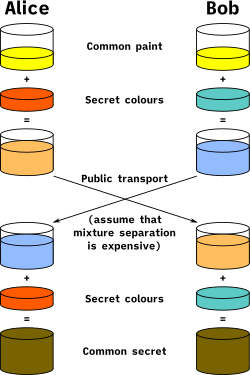
\includegraphics{/home/oxio2/Documenti/obsidian-vault/Epico/diffie_hellman.png}

\begin{center}\rule{0.5\linewidth}{0.5pt}\end{center}

\hypertarget{references-8}{%
\section{References}\label{references-8}}

Gli Algoritmi di Cifratura che utilizzano una o più chiavi seguono il
Teorema di Kerckhoff, cioè che la sicurezza di un algoritmo è dato dalla
chiave, non dall'algoritmo

202303270927\\
Status:\\
Tags: Sistemi

\hypertarget{teorema-di-kerckhoff}{%
\section{Teorema di Kerckhoff}\label{teorema-di-kerckhoff}}

Il \textbf{teorema di Kerchoff} è un principio fondamentale della
Crittografia moderna che afferma che la sicurezza di un Cifrante non
deve basarsi sulla segretezza dell'Algoritmo di Cifratura, ma piuttosto
sulla Chiave di Cifratura.

Così facendo è possibile rendere l'Algoritmo pubblico per studiare la
sua sicurezza più a fondo e nel caso la Chiave di Cifratura venga
violata, non è necessario realizzare un nuovo Algoritmo, ma basta
semplicemente cambiare Chiave di Cifratura.

\begin{center}\rule{0.5\linewidth}{0.5pt}\end{center}

\hypertarget{references-9}{%
\section{References}\label{references-9}}

Altri principi di Crittografia sono:

\begin{itemize}
\tightlist
\item
  Confusione
\item
  Diffusione
\end{itemize}

202303270932\\
Status:\\
Tags: Sistemi

\hypertarget{confusione}{%
\section{Confusione}\label{confusione}}

Nella Crittografia, la \textbf{Confusione} si riferisce alla capacità di
rendere la relazione tra la Chiave di Cifratura e il testo in chiaro il
più complessa possibile, in modo che sia difficile dedurre la chiave a
partire dal testo cifrato.

\begin{center}\rule{0.5\linewidth}{0.5pt}\end{center}

\hypertarget{references-10}{%
\section{References}\label{references-10}}

ChatGPT

\hfill\break

202303270934\\
Status:\\
Tags:Sistemi

\hypertarget{diffusione}{%
\section{Diffusione}\label{diffusione}}

Nella Crittografia, la \textbf{Diffusione} si riferisce alla capacità di
distribuire le informazioni sulla chiave in tutto il testo cifrato, in
modo che una piccola modifica nella chiave produca una grande variazione
nel testo cifrato

\begin{center}\rule{0.5\linewidth}{0.5pt}\end{center}

\hypertarget{references-11}{%
\section{References}\label{references-11}}

ChatGPT

\hypertarget{esempi}{%
\paragraph{Esempi}\label{esempi}}

Un esempio di Algoritmo di Cifratura utilizzato durano il IX Secolo è il
Cifrario a Campale Germanico, utilizzato dalle forze armate Tedesche
durante la Prima Guerra Mondiale.

{Cifrario a Campale Germanico}

Un'altro esempio di Algoritmo di Cifratura è quello utilizzato dalla
macchina Enigma, utilizzato dalle forze armate Tedesche durante la
Seconda Guerra Mondiale

202303270836\\
Status:\\
Tags:Sistemi Crittografia

\hypertarget{enigma}{%
\section{Enigma}\label{enigma}}

\textbf{Enigma} è un dispositivo Cifrante Elettromeccanico utilizzato
dalle forze armate Tedesche durante la Seconda Guerra Mondiale per
Cifrare e Decifrare messaggi.

I componenti della macchina sono:

\begin{itemize}
\tightlist
\item
  Una tastiera composta dalle 26 lettere dell'alfabeto utilizzato per
  inserire le lettere.
\item
  Una "lamp board", composta da una serie di lampadine disposte in una
  griglia corrispondente alla tastiera della macchina e utilizzato per
  visualizzare ciascun carattere decifrato per ciascun carattere immessi
  dalla tastiera.
\item
  Dei rotori che girando progressivamente ad ogni input da tastiera
  cifra o decifra il carattere immesso da tastiera.
\item
  Una plugboard(o pannello di controllo), composta da una piastra con
  prese per cavi, dove i cavi possono essere inseriti nelle prese per
  scambiare le coppie di lettere.
\item
  Una batteria interna per alimentare la macchina, rendendola così
  portabile
\end{itemize}

La chiave di cifratura della macchina \textbf{Enigma} è composta da:

\begin{itemize}
\tightlist
\item
  L'ordine della posizione dei rotori
\item
  Ring settings, cioè la rotazione iniziale di ogni rotore.
\item
  Configurazione della plugboard, cioè dei cavi che scambiano le coppie
  di lettere.
\end{itemize}

Il componente fondamentale della macchina \textbf{Enigma} sono i rotori,
cioè dischi metallici sottili con 26 contatti elettrici corrispondenti
alle 26 lettere dell'alfabeto latino su ambo i lati.\\
I rotori vengono posizionati uno accanto all'altro con i contatti uniti,
in modo che il segnale passasse attraverso i contatti di tutti i rotori
per poi tornare indietro.\\
Ad ogni carattere immesso da tastiera, il primo rotore avanza di una
posizione e quando completa il giro fa avanzare il rotore successivo.\\
In questo modo i contatti elettrici e il carattere che ne risulta cambia
ad ogni immissione da tastiera.

\begin{center}\rule{0.5\linewidth}{0.5pt}\end{center}

\hypertarget{references-12}{%
\section{References}\label{references-12}}

Youtube -\textgreater{}
\href{https://www.youtube.com/watch?v=ybkkiGtJmkM}{How did the Enigma
Machine work?}

202303251429\\
Status:\\
Tags: Sistemi Cifratura

\hypertarget{cifrario-di-feistel}{%
\section{Cifrario di Feistel}\label{cifrario-di-feistel}}

Il \textbf{Cifrario di Feistel} è un Algoritmo di Cifratura A Blocchi
che ha preso il nome di Rete di Feistel.\\
Moltissimi algoritmi di Cifratura a Blocchi la utilizzato, incluso il
famoso Data Encryption Standard(DES).

\begin{enumerate}
\tightlist
\item
  L'algoritmo divide il dato in due parti (uguali o non), la parte
  destra prende il nome di {\(L\)} e la parte sinistra prende il nome di
  {\(R\)}.
\item
  Primo passaggio

  \begin{enumerate}
  \tightlist
  \item
    Al blocco posto a sinistra (cioè {\(L\)}) viene effettuata una
    funzione di Cifratura in base all'Algoritmo utilizzato, viene
    effettuato uno XOR({\(\oplus\)}) ,con il blocco posto a destra (cioè
    {\(R\)}) e infine spostato a destra. Matematicamente viene denoto
    come {\(L \oplus f(R,k_{1})\)} dove {\(k_{1}\)} equivale alla chiave
    numero 1
  \item
    Il blocco a destra (cioè {\(R\)}) viene spostato a sinistra
  \end{enumerate}
\item
  Secondo passaggio

  \begin{enumerate}
  \tightlist
  \item
    Al blocco posto a sinistra (cioè {\(R\)}) viene effettuata una
    funzione di Cifratura in base all'Algoritmo utilizzato, viene
    effettuato uno XOR({\(\oplus\)}) ,con il blocco posto a destra (cioè
    {\(\oplus f(R,k_{1})\)}) e infine spostato a destra. Matematicamente
    viene denoto come {\(R \oplus f(L \oplus f(R,k_{1}),k_{2}\rbrack\)}
    dove {\(k_{1}\)} equivale alla chiave numero 2
  \item
    Il blocco a destra (cioè {\(\oplus f(R,k_{1})\)}) viene spostato a
    sinistra
  \end{enumerate}
\item
  Terzo passaggio: I due blocchi vengono scambiati di posto

  \begin{enumerate}
  \tightlist
  \item
    Il blocco a sinistra (cioè {\(L \oplus f(R,k_{1})\)}) viene posto a
    destra
  \item
    Il blocco a destra (cioè
    {\(R \oplus f(L \oplus f(R,k_{1}),k_{2}\rbrack\)}) viene spostato a
    sinistra
  \end{enumerate}
\end{enumerate}

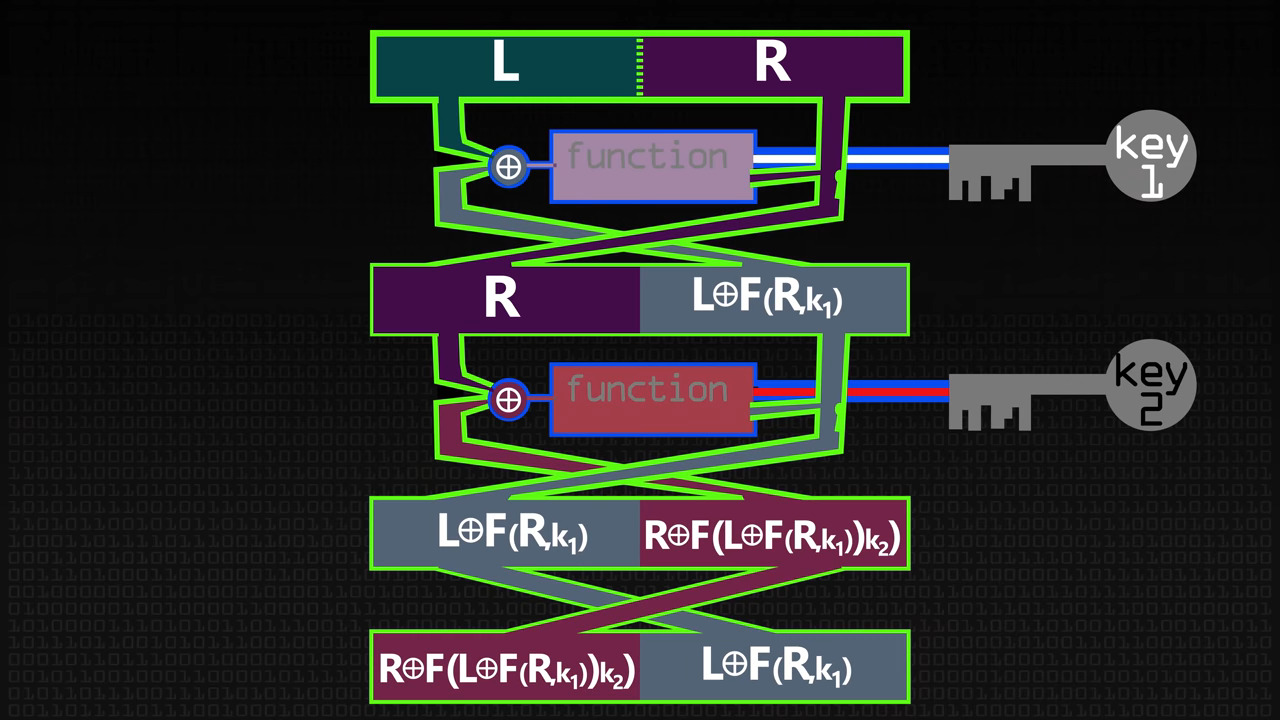
\includegraphics{/home/oxio2/Documenti/obsidian-vault/Epico/feistel.jpeg}

Per compiere la decifratura:

\begin{enumerate}
\tightlist
\item
  L'algoritmo divide il dato in due parti (uguali o non), la parte
  destra prende il nome di {\(L\)} e la parte sinistra prende il nome di
  {\(R\)}.
\item
  Primo passaggio

  \begin{enumerate}
  \tightlist
  \item
    Al blocco posto a sinistra (cioè
    {\(R \oplus f(L \oplus f(R,k_{1}),k_{2})\)}) viene effettuata una
    funzione di Cifratura in base all'Algoritmo utilizzato, viene
    effettuato uno XOR({\(\oplus\)}) ,con il blocco posto a destra (cioè
    {\(L \oplus f(R,k_{1})\)}) e infine spostato a destra.
    Matematicamente viene denoto a seguito di Semplificazione come
    {\(L \oplus F(R,k_{1})\)} dove {\(k_{1}\)} equivale alla chiave
    numero 1
  \item
    Il blocco a destra (cioè {\(L \oplus F(R,k_{1})\)}) viene spostato a
    sinistra
  \end{enumerate}
\item
  Secondo passaggio

  \begin{enumerate}
  \tightlist
  \item
    Al blocco posto a sinistra (cioè
    {\(L \oplus F(L \oplus f(R,k_{1}))\)}) viene effettuata una funzione
    di Cifratura in base all'Algoritmo utilizzato, viene effettuato uno
    XOR({\(\oplus\)}) ,con il blocco posto a destra (cioè {\(R\)}) e
    infine spostato a destra. Matematicamente viene denoto a seguito di
    Semplificazione come {\(L\)} dove {\(k_{1}\)} equivale alla chiave
    numero 2
  \item
    Il blocco a destra (cioè {\(R\)}) viene spostato a sinistra
  \end{enumerate}
\item
  Terzo passaggio: I due blocchi vengono scambiati di posto

  \begin{enumerate}
  \tightlist
  \item
    Il blocco a sinistra (cioè {\(R\)}) viene posto a destra
  \item
    Il blocco a destra (cioè {\(L\)}) viene spostato a sinistra
  \end{enumerate}
\end{enumerate}

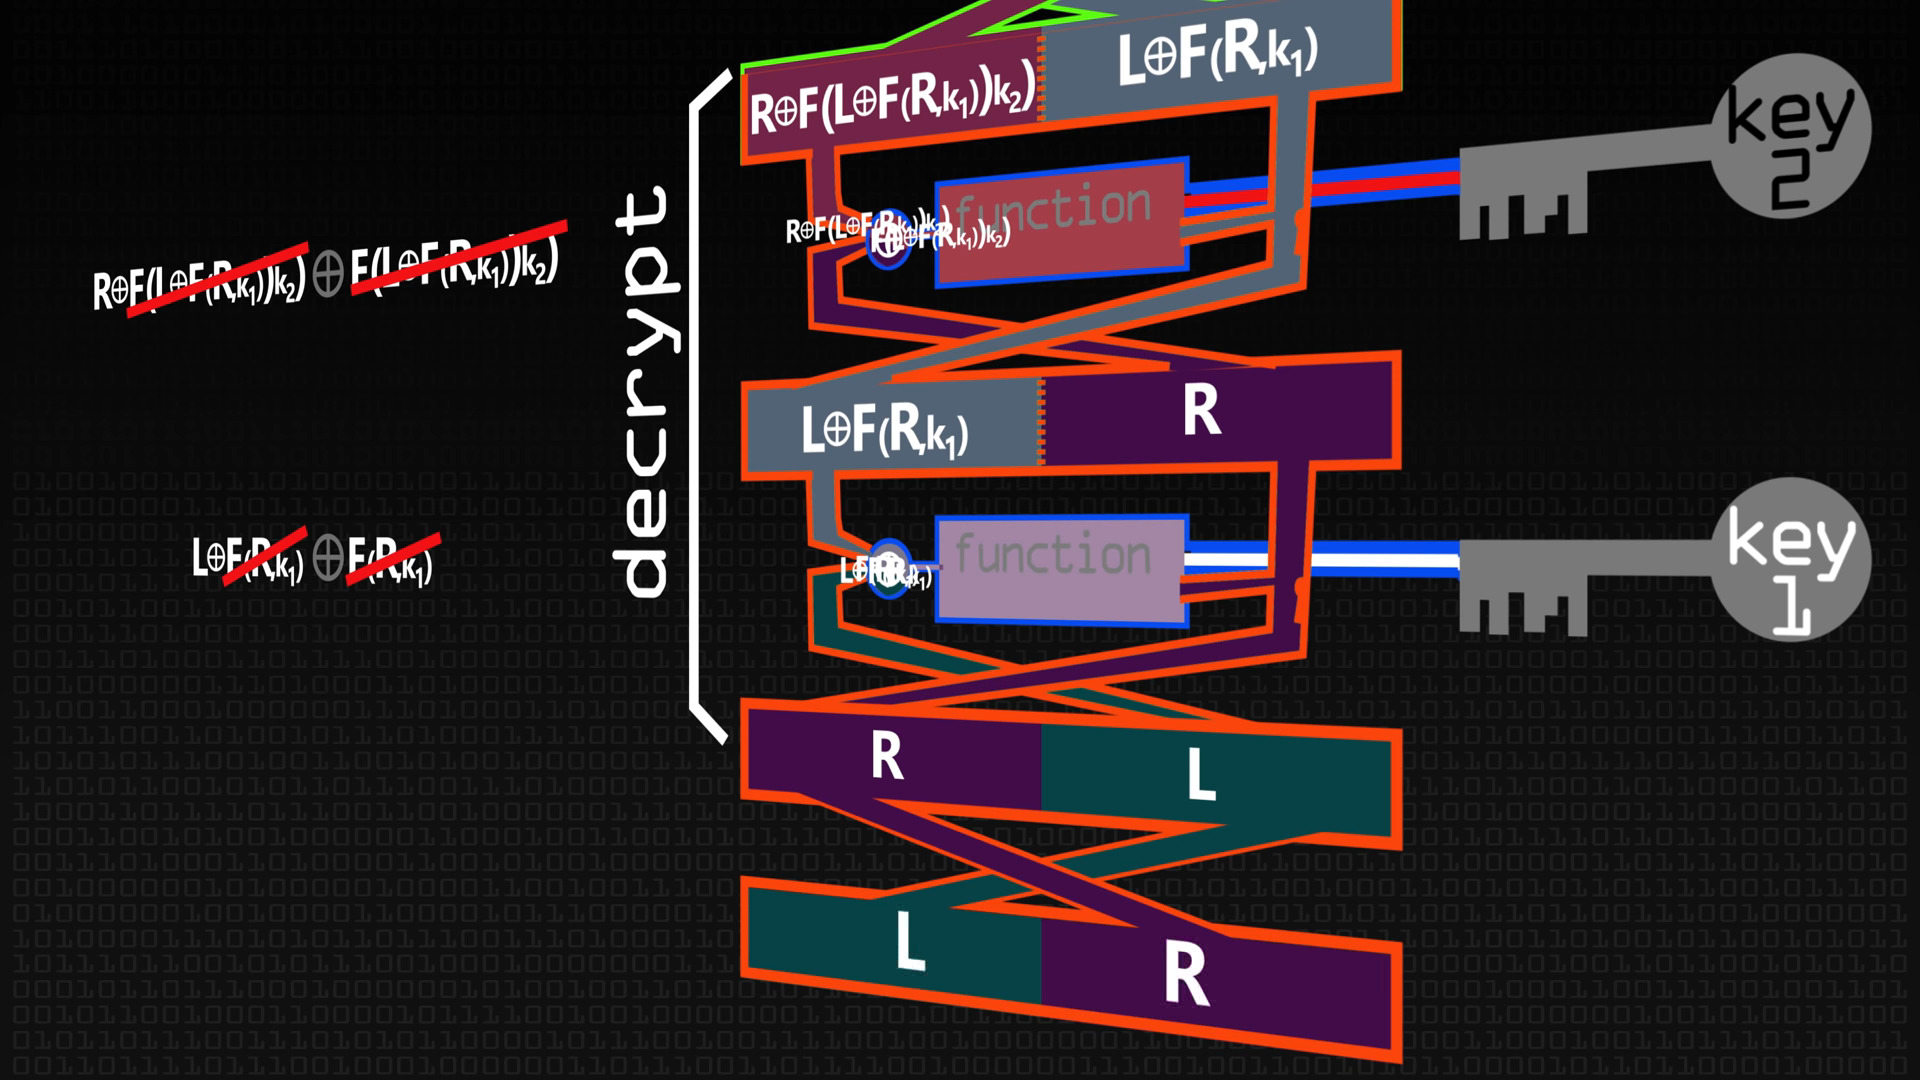
\includegraphics{/home/oxio2/Documenti/obsidian-vault/Epico/feistel_decypher.jpeg}

\begin{center}\rule{0.5\linewidth}{0.5pt}\end{center}

\hypertarget{references-13}{%
\section{References}\label{references-13}}

\hfill\break

202303250021\\
Status:\\
Tags: Sistemi

\hypertarget{data-encryption-standard}{%
\section{Data Encryption Standard}\label{data-encryption-standard}}

Il Data Encryption Standard è un Algoritmo di Cifratura pubblicato nel
1977 e standardizzato nel 1977.

La chiave è formata da 64 bit ed è divisa in

\begin{itemize}
\tightlist
\item
  56 bit di chiave effettiva
\item
  8 bit di parità (ogni ottavo bit della chiave è un bit di parità)
\end{itemize}

L'Algoritmo prevede 16 round di Trasposizioni successive.\\
Non lavora su un alfabeto di 26 caratteri ma su file binari con byte
codificati in ASCII, quindi 128 caratteri, dei quali solo 96 sono
definiti stampabili (non sono caratteri speciali)

\begin{enumerate}
\tightlist
\item
  Il testo di 64 bit viene suddiviso in blocchi di 8 byte e codificato
  in ASCII per ottenere una Stringa di 64 cifre binarie
\item
  Avviene una Permutazione iniziale {\(IP\)} dei 64 bit
\item
  Si compiono 16 round dell'Algoritmo di Cifratura "Cifrario di
  Feistel".
\item
  Avviene una Permutazione finale inversa a quella iniziale, cioè
  {\(FP = IP^{- 1}\)}
\end{enumerate}

\hypertarget{png}{%
\subsection{\texorpdfstring{\protect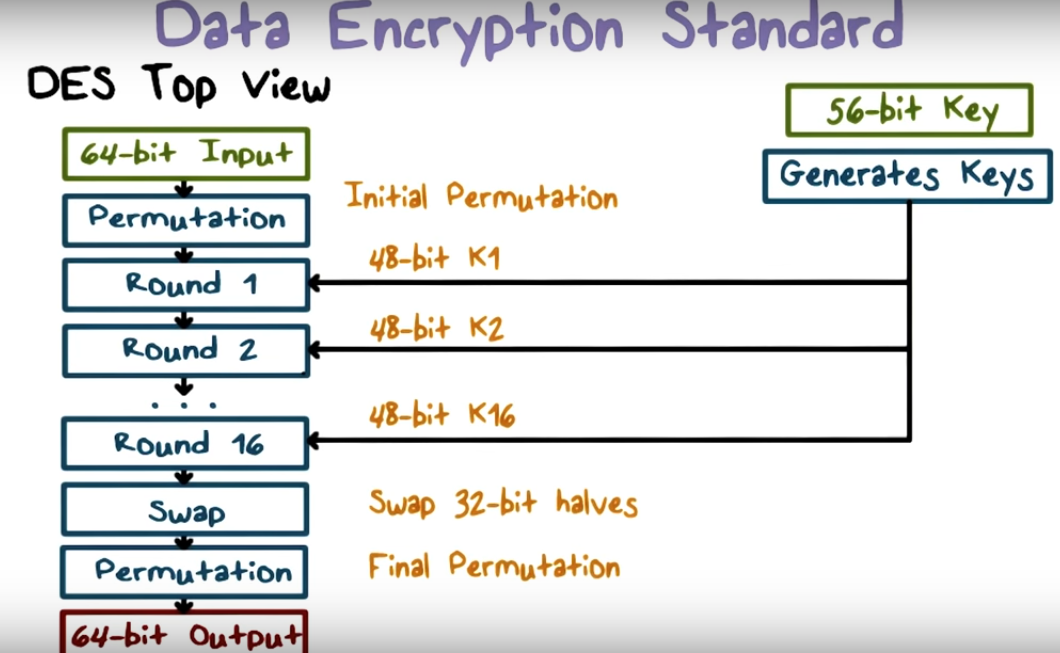
\includegraphics{/home/oxio2/Documenti/obsidian-vault/Epico/2023-03-25_00-54.png}}{2023-03-25\_00-54.png}}\label{png}}

\hypertarget{references-14}{%
\section{References}\label{references-14}}

ChatGPT\\
Computerphile \href{https://www.youtube.com/watch?v=FGhj3CGxl8I}{Feistel
Cipher - Computerphile}

\end{document}
